%%%%%%%%%%%%%%%%%%%%%%%%%%%%%%%%%%%%%%%%%%%%%%%%%%%%%%%%%%%%%%%%%%%%%%%%
% Plantilla TFG/TFM
% Escuela Politécnica Superior de la Universidad de Alicante
% Realizado por: Jose Manuel Requena Plens
% Contacto: info@jmrplens.com / Telegram:@jmrplens
%%%%%%%%%%%%%%%%%%%%%%%%%%%%%%%%%%%%%%%%%%%%%%%%%%%%%%%%%%%%%%%%%%%%%%%%

\chapter{Estado del arte}

\section{La demoscene}

\subsection{Qué es la demoscene}

La \emph{demoscene} es una subcultura informática cuyo principal objetivo es la creación de demostraciones técnicas llamadas \emph{demoscenes}. Una \emph{demoscene} es un programa autocontenido y por norma general de peso ligero que intenta explotar al máximo el \emph{software} y el \emph{hardware} de la máquina que la ejecuta, con el fin de generar efectos visuales y sonoros. El objetivo de una \emph{demoscene} suele consistir en mostrar el ingenio y las habilidades del programador, así como tratar de impresionar al público.\\

Además, aunque el \emph{demoscening} en sí mismo no se puede considerar una forma de arte, sí que es cierto que muchas demos poseen un cierto componente artístico.\\ 

Se distinguen principalmente dos tipos de demo\footnote{\url{http://www.oldskool.org/demos/explained/demo_reference.html}}:

\begin{itemize}
  \item \textbf{Demo}: programa que genera gráficos y sonido en tiempo real. Suele tener una extensión superior a 5 minutos y normalmente no tienen límite de tamaño. Una demo suele ser creada por un grupo de personas que incluye al menos un programador, un diseñador gráfico y un músico. Las demos actuales suelen estar realizadas en 3D y cuentan con aceleración gráfica por hardware. Las demos más antiguas o realizadas para plataformas más antiguas (conocidas como "demos \emph{oldskool}") son procesadas de forma íntegra por la CPU (pues las plataformas para las que se desarrollan no poseen GPU) y suelen combinar ilusiones 3D con efectos gráficos en 2D.
  \item \textbf{Intro}: una demo de corta duración. Una intro suele ser temática (mientras que una demo suele compilar distintas escenas/temáticas). Además, las intros no suelen superar los 5 minutos de duración y su tamaño tiende a estar restringido. Las principales categorías de intros son 64K (65536 bytes), 4K (4096 bytes) y 1K (1024 bytes).
\end{itemize}

Existen otras categorías de demo, aunque son mucho menos comunes, como las \textbf{mega demos} (demos de gran duración/extensión, compuestas por múltiples partes) o las \textbf{dentros} (intros cuyo propósito es ofrecer un avance de una demo por llegar, todavía en desarrollo).\\

Además, existen muchas otras categorías derivadas o relacionadas con la \emph{demoscene}, como la creación de gráficos procedimentales. Una de las subcategorías más populares dentro de esta son las \textbf{4K images}, imágenes complejas y de alta resolución generadas procedimentalmente por programas de 4096 bytes. También es posible encontrar categorías similares relacionadas con la generación procedimental de archivos de música o vídeo. Las mayores diferencias entre estas producciones y las demos son su tiempo de ejecución (no se ejecutan en tiempo real) y las técnicas que usan (al no ser el tiempo una limitación, pueden usar algoritmos computacionalmente más costosos, pero que generan resultados más complejos).

\subsection{Orígenes de la demoscene}

A principios de los años 80, con la popularización de los primeros ordenadores personales, la computación dejó de ser algo que sucedía en universidades para pasar a abrirse al gran mercado. Con ello, llegó también la distribución del software, aunque en aquella época no se producía por internet, si no tan sólo por medios físicos, como los disquetes. Estos programas venían con protecciones de copia por parte de los desarrolladores para evitar su distribución ilegal. Poco tardaron, no obstante, en aparecer los primeros \emph{crackers}, personas que se dedicaban a eliminar las protecciones de copia del software para su distribución gratuita. Esto llevó a la creación de una subcultura informática basada en el \emph{cracking} de videojuegos y otros tipos de software, al margen de la legalidad. Esto se hacía no solo con la intención de poder ditribuir el software de forma gratuita, si no que también suponía una fuente de diversión y competición para los \emph{crackers}\footnote{\url{https://web.archive.org/web/20170726063815/http://tomaes.32x.de/text/faq.php\#2.3}}.\\

Es por ello que los denominados \emph{crackers} empezaron a "firmar" el software que \emph{crackeaban} con seudónimos que aparecían en los menús o en las intros de los juegos. Con el tiempo, la competición y la ambición de los \emph{crackers} fue aumentando, y llegó un punto en el que no solo se limitaban a quitar las protecciones de copia del software, si no que también creaban sus propias intros para los programas.\\

Es en este punto cuando la \emph{demoscene} empieza a tomar forma, cuando una parte de los \emph{crackers} deciden retornar a la legalidad pero sin dejar atrás la competición y la diversión. De este modo, este nuevo sector se empieza a dedicar a la creación de intros y demos cuyo objetivo es mostrar sus habilidades al resto de \emph{demosceners}\footnote{\url{http://widerscreen.fi/assets/reunanen-wider-1-2-2014.pdf}}.

\subsection{Composición y cultura de la demoscene}

La \emph{demoscene} es una subcultura informática muy centrada en el trabajo en equipo y en compartir. Con el desarrollo y popularización de la \emph{demoscene}, a partir de principios de los 90 se popularizó y se estandarizó, con la creación de eventos y competiciones.\\

Heredado de las \emph{copyparties}, eventos en los que \emph{crackers} y \emph{demosceners} se juntaban para conocerse y compartir software, al margen de la legalidad, nuevos eventos empezaron a crearse a principios de los noventa. Estos eventos sí eran legales y se centraban únicamente en el aspecto de las demos. Pasan a ser eventos sociales en los que los \emph{demosceners} se conocen, comparten y compiten.\\

Estos eventos, conocidos como \emph{demoparties}, pasan entonces a ser concursos y tener distintas categorías y premios. Para concursar, normalmente los competidores se juntaban en grupos, usualmente compuestos por al menos un programador, un diseñador gráfico y un músico. Estos grupos tenían su propio nombre e identidad. A su vez, cada uno de los componentes del grupo también solía usar un seudónimo. El uso de un seudónimo es una herencia de los orígenes de la \emph{demoscene} en el \emph{cracking}, aunque el propósito de usar un alias cambia. Mientras que los \emph{crackers} usaban un nombre falso para ocultar su identidad, pues realizaban actividades ilegales, los \emph{demosceners} usan este alias como una forma de expresión.

\subsection{La demoscene en la actualidad}

Si bien la \emph{demoscene} siempre se ha mantenido como una subcultura y nunca ha llegado a tener una popularidad masiva, su auge se dio en los años noventa.  En la actualidad, muchos de los eventos de \emph{demoscening} que se crearon en los 90 han desaparecido, y otros tantos han derivado en eventos dedicados a los ordenadores de forma mucho más genérica, derivando en eventos de software o en \emph{LAN-parties}.\\

Del mismo modo que muchas ferias y eventos han desaparecido, muchos otros también se han ido creando. No obstante, parece que hay una tendencia general hacia el olvido.\\

Las \emph{demoparties} en la actualidad suelen ser eventos locales, normalmente humildes, donde participan apasionados y nostálgicos.\\

Es difícil atribuir las causas de la lenta caída en popularidad de la \emph{demoscene}, aunque hay varios factores que pueden contribuir a ello, del mismo modo que hay una serie de factores que evitan que se pierda.\\

Por un lado, la \emph{demoscene} es cada vez más pequeña debido a:

\begin{itemize}
  \item Siempre ha sido una subcultura, y nunca ha destacado especialmente por encima de otras subculturas informáticas.
  \item Para poder participar en la \emph{demoscene} hace falta una gran cantidad de conocimiento matemático y de programación de bajo nivel, cualidades que no abundan.
  \item Con el auge de los ordenadores, otro tipo de espacios más accesibles al público como las ferias tecnológicas, las ferias de videojuegos o las ferias de programación han eclipsado parcialmente a la \emph{demoscene}.
  \item Una parte de los \emph{demosceners} eran reacios a la incorporación de gente nueva e inexperta a la \emph{demoscene}, pues si bien aportaban sangre nueva, sus metas y conocimiento se alejaban de los originales de la escena.
\end{itemize}

Todos estos factores han contribuido a colocar la \emph{demoscene} como una práctica de nicho. Quizá una crítica válida sería que no ha sabido adaptarse de forma conveniente a los nuevos tiempos. El mundo de la \emph{demoscene} no ha sabido publicitarse o venderse suficientemente bien como para llegar a ser conocido por un público mayor. Sin embargo, la \emph{demoscene} sigue viva, y estos son algunos de los factores que contribuyen a ello:

\begin{itemize}
	\item El auge de lo \emph{retro}. En esta última década ha empezado a masivizarse un cierto reconocimiento y nostalgia hacia los orígenes de la computación y del videojuego. La popularización de los juegos \emph{indie}, técnicas como el \emph{pixel art} y tributos a videojuegos antiguos han llevado a destapar obras olvidadas y a suscitar un nuevo interés por todo lo \emph{retro}.
	\item La pasión y dedicación de los \emph{demosceners}, que siguen produciendo y compartiendo su obra, extendiendo así su pasión y abriéndola al público general.
	\item La masivización de la informática. Hoy en día hay muchísimos más informáticos que en los años 80 y 90. Si bien es cierto que hay una tendencia de abandono hacia el bajo nivel, también hay mucha más gente que se hace preguntas, investiga y se interesa por el mismo.
\end{itemize}

Como reflexión final me gustaría añadir que creo que es posible mantener el panorama de la \emph{demoscene} vivo, pero pienso que esto va a ser muy complicado si no se intenta abrir al público, cosa que algunas \emph{demoparties} ya están haciendo. Está claro que al abrir la \emph{demoscene} al público general se pierden cosas por el camino, y se gana gente que tiene un interés mucho más casual y mucho menos pasional. Creo que en el panorama actual esa gente es necesaria. No todo el mundo tiene el tiempo o la capacidad como para meterse de lleno en la \emph{demoscene}, pero hay muchas personas que sí pueden tener curiosidad por ella de una forma mucho más básica, y esta gente también cuenta. Cada vez es más común encontrar en ferias de videojuegos puestos \emph{retro}, y hay incluso museos del videojuego. La nostalgia y la veneración por los orígenes se abre paso, y pienso que es en este lugar donde la \emph{demoscene} puede buscar su camino.

\section{Eventos de demoscening}

A continuación se listan y describen brevemente algunas \emph{demosparties} que aún se celebran en la actualidad, en el año 2019.

\begin{itemize}
	\item \textbf{Revision}: tiene lugar en durante Pascua, en Alemania. Es la sucesora de la \emph{demoparty} Breakpoint\footnote{\url{http://breakpoint.untergrund.net}}. El evento se estableció en 2011, tras el fin de Breakpoint, y mantiene a muchos de los organizadores. El evento congrega a más de 800 personas de todo el mundo cada año, y es el mayor evento dedicado exclusivamente a la \emph{demoscene} en el mundo \footnote{\url{https://2019.revision-party.net}}.
	\item \textbf{Assembly} [\ref{fig:assembly}]: tiene lugar en verano en Finlandia, y es el mayor evento de \emph{demoscening} en el país. Además, es uno de las \emph{demoparties} más antiguas que siguen en activo, cumpliendo 25 años el pasado 2017. Sin embargo, el evento no está dedicado exclusivamente a la \emph{demoscene}, si no que es también un evento de videojuegos y \emph{esports}. No obstante, la \emph{demoscene} sigue siendo importante en él, y se celebran anualmente concursos en 5 categorías distintas (Demo, Oldskool demo, 64K intro, 4K intro y 1K intro)\footnote{\url{https://www.assembly.org/summer19/demoscene}}.
	\item \textbf{VIP (Very Important Party)}: es la \emph{demoparty} más longeva de Francia, cumpliendo este año su 20 aniversario. Congrega a personas de todas partes de Europa, aunque es una \emph{demoparty} principlamente francesa\footnote{\url{https://en.wikipedia.org/wiki/Very_Important_Party}}. Fue fundada por el grupo de \emph{demosceners} \emph{PoPsY TeAm}\footnote{\url{http://www.popsyteam.org}}.
	\item \textbf{Nova}: esta \emph{demoparty} fue creada en 2017, por lo que este año se celebra su tercera edición. Es la mayor \emph{demoparty} en Reino Unido, con una salón principial con capacidad para hasta cien \emph{demosceners}\footnote{\url{http://www.novaparty.org}}.
	\item  \textbf{Alternative Party}: es uno de los eventos de \emph{demoscening} más grandes de Finlandia. Es un festival bastante peculiar, (o alternativo, como su nombre indica) y su objetivo es motivar a los programadores y artistas a explorar su creatividad y nuevos puntos de vista. Suele mezclar ordenadores de distintas épocas y capacidades. Aunque mantiene una categoría constante a la mejor demo, el resto de categorías y premios cambian cada año, suponiendo así un reto aún mayor para los programadores. Ha tenido distintos invitados célebres dentro del mundo de la informática, como Al Lowe, creador del juego \emph{Leisure Suit Larry}. Además, la primera noche del evento incluye un concierto de música en el que participan artistas del mundo de la \emph{demoscene}. Este año se celebra su 20 aniversario\footnote{\url{http://www.altparty.org}}. 
	\item \textbf{Chaos Constructions}: es el festival de \emph{demoscenes} más longevo y popular que se celebra en Rusia. Tiene lugar en verano y se creó en 1995, aunque en aquel momento se llamada \emph{Enlight}. La celebración de esta \emph{demoparty} en el año 1997 congregó a más de 1200 personas. En la actualidad, su temática se ha ampliado, incluyendo nuevas areas como exposiciones y charlas empresariales. En 2018, el festival tuvo lugar durante dos días sin interrupción, contó con participantes internacionales y se emitió de forma íntegra por \emph{Twicht}\footnote{\url{https://chaosconstructions.ru/en/}}
\end{itemize}

\begin{figure}[h]
	\centering
	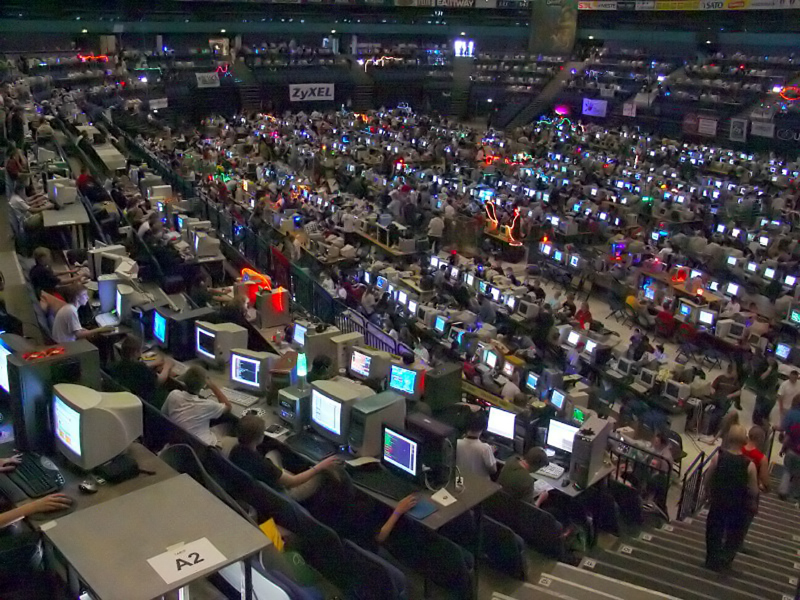
\includegraphics[width=10cm]{archivos/Assembly2004}
	\caption{Assembly 2004 - Fuente: \href{https://en.wikipedia.org/wiki/Demoscene\#/media/File:Assembly2004-areena01.jpg}{Wikipedia}}
	\label{fig:assembly}
\end{figure}

\section{Grupos de demoscening}

A continuación se listan y describen brevemente algunos de los grupos de \emph{demosceners} más populares.

\subsection{Farbrausch}

Farbraush es un grupo de \emph{demosceners} de origen alemán que empezó a ser notado a partir de diciembre del 2000, con su octava producción, llamada \emph{fr-08: .the .product}\footnote{\url{http://www.farbrausch.de/prod&which=17.py}}.\\

El nombre del grupo se puede traducir como "éxtasis de color". Todos sus proyectos empiezan por "fr-número\_del\_proyecto", donde el número del proyecto se decide en el momento de empezar a trabajar en el mismo, independientemente de cuándo se produzca su lanzamiento.\\

Farbraush tiene un gran cantidad de demos notorias, como Debris [\ref{fig:debris}], que está considerada en el popular portal \emph{demoscener} \url{http://www.pouet.net} como la mejor demo de todos los tiempos.

\begin{figure}[h]
	\centering
	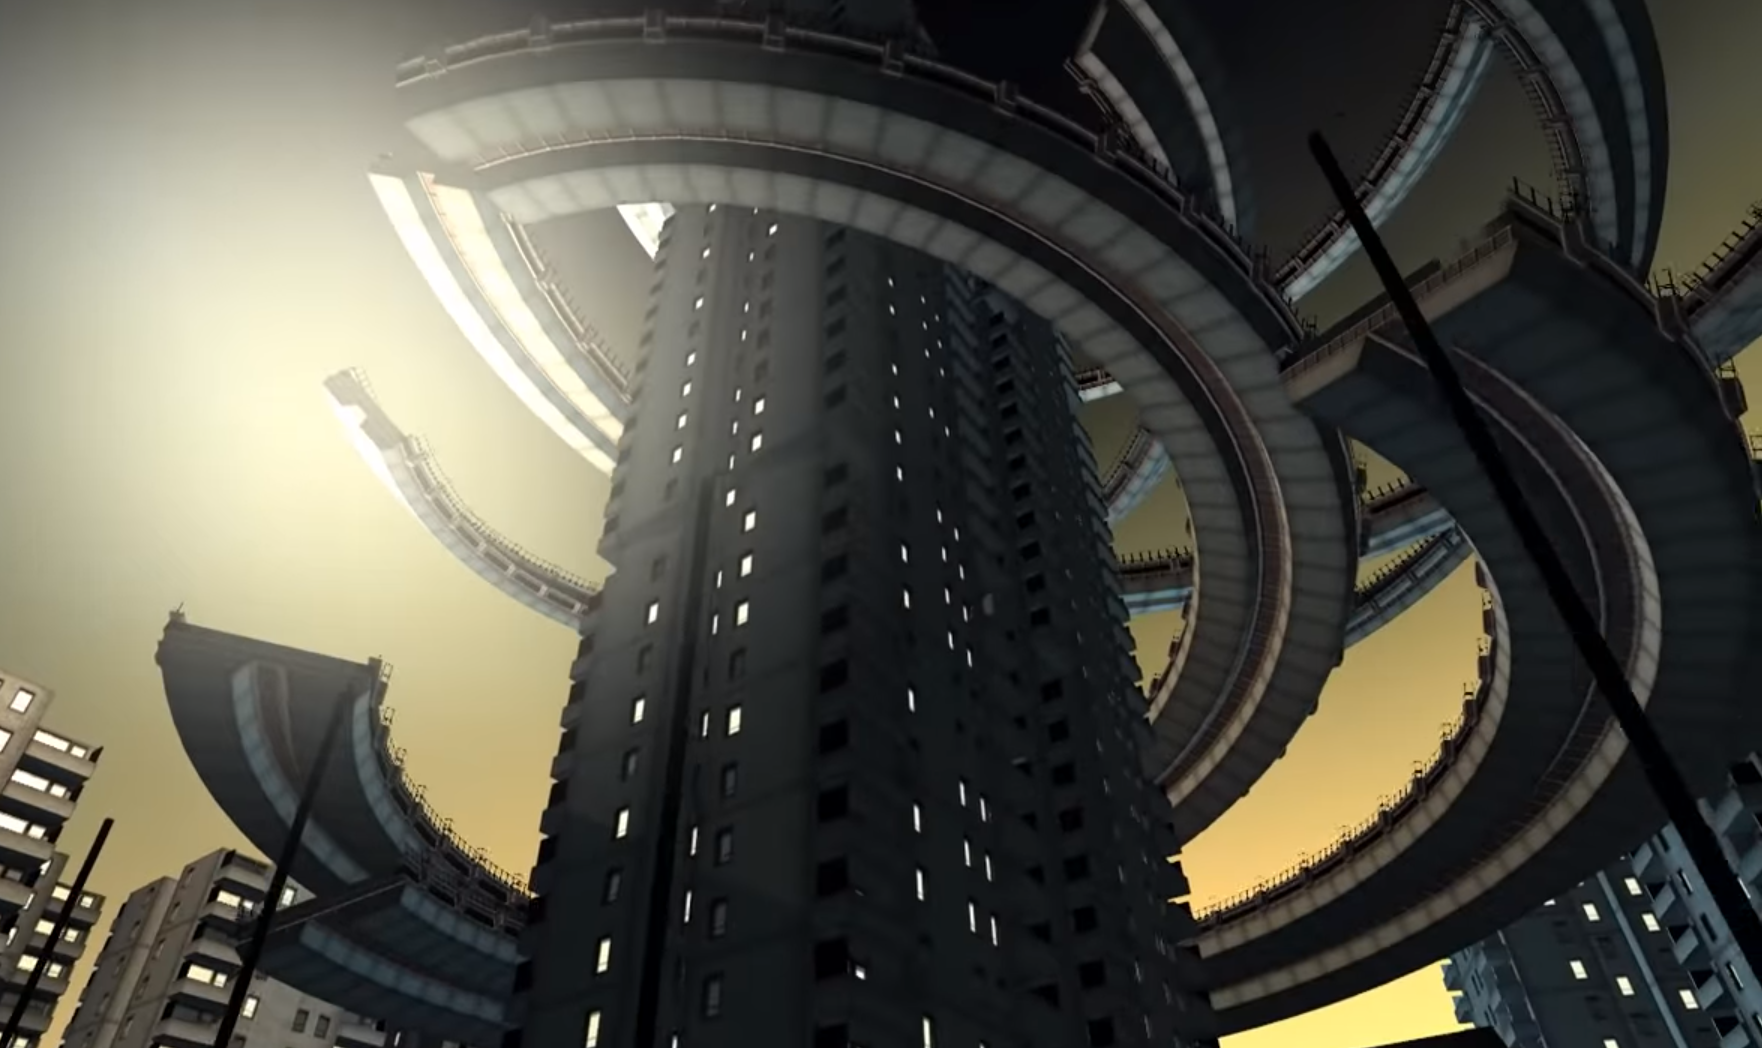
\includegraphics[width=10cm]{archivos/fr-041-debris}
	\caption{Farbrausch 41: Debris - Fuente: \href{https://www.youtube.com/watch?v=jY5Vrc5G0lk}{YouTube}}
	\label{fig:debris}
\end{figure}

Además, en el año 2004 un subgrupo dentro de Farbrausch, denominado \emph{.theprodukkt}, lanzó \emph{.kkrieger}, un juego de disparos en primera persona que ocupaba tan sólo 96kB. Este pequeño tamaño se consiguió mediante el uso de generación procedimental para las texturas y el uso de formas básicas (cubos, esferas...) combinados y deformados para los modelos. El juego [\ref{fig:kkrieger}] recibió distintos premios y fue alabado por la comunidad.\\

\begin{figure}[h]
	\centering
	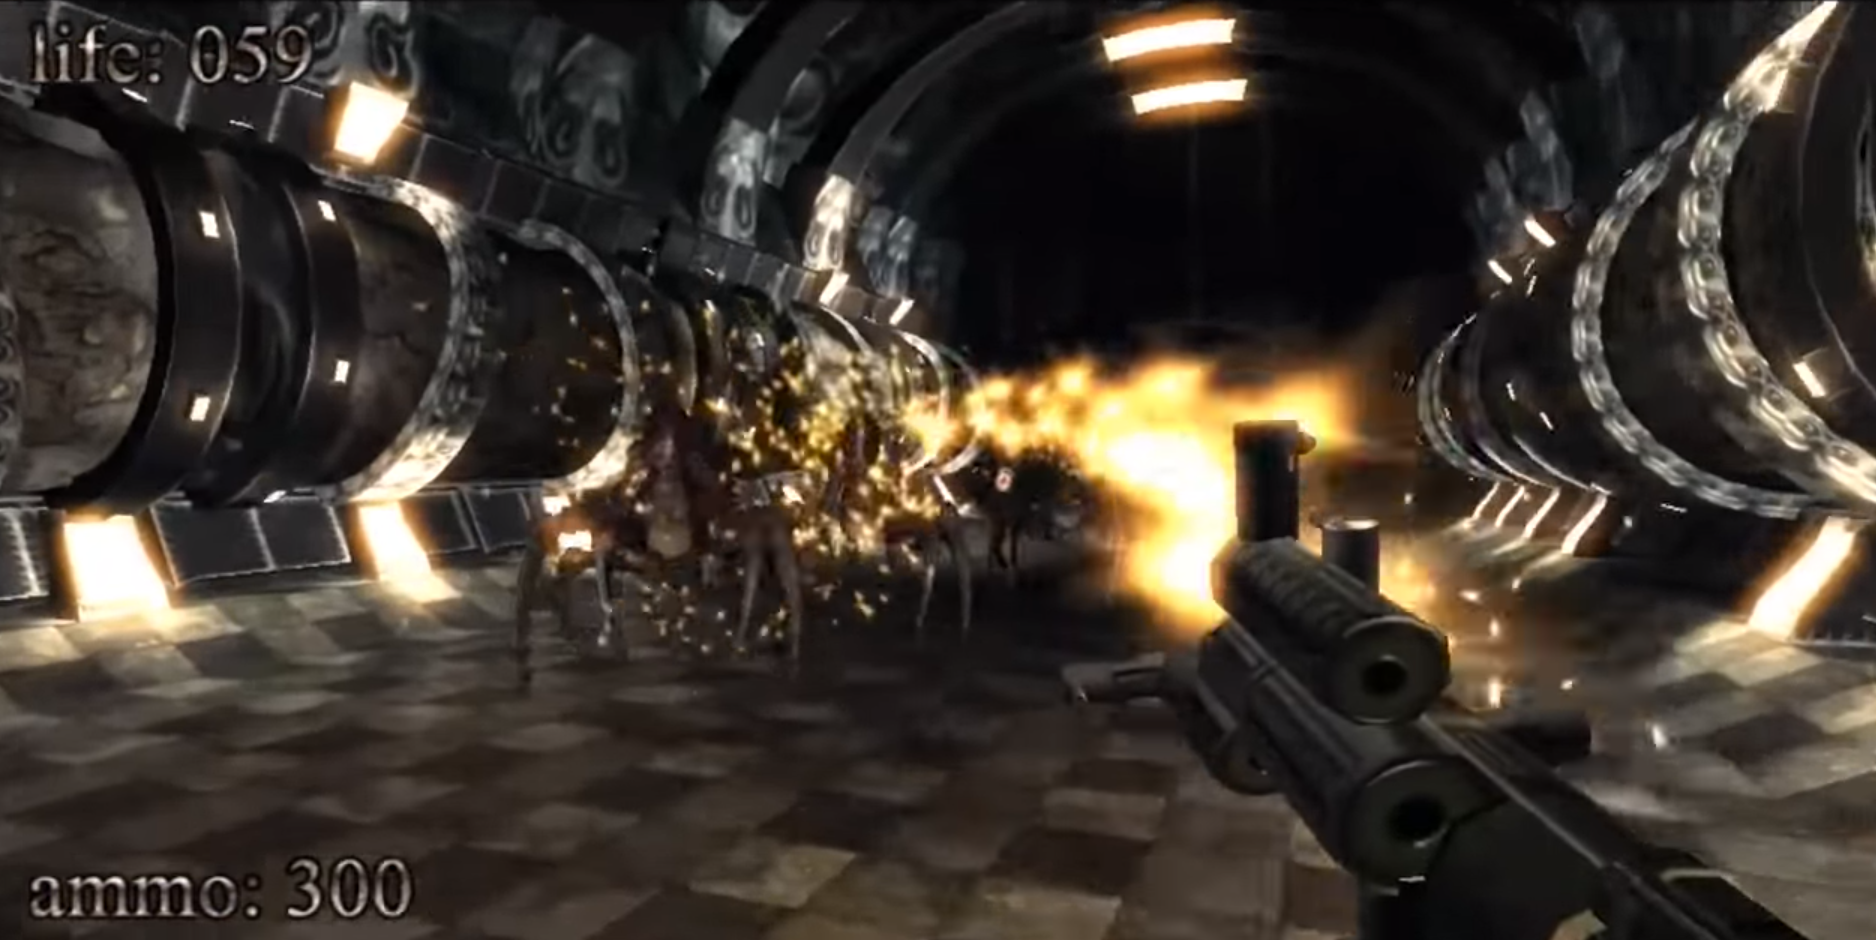
\includegraphics[width=10cm]{archivos/kkrieger}
	\caption{Videojuego de 96kB: .kkrieger - Fuente: \href{https://www.youtube.com/watch?v=2NBG-sKFaB0}{YouTube}}
	\label{fig:kkrieger}
\end{figure}

El grupo sigue en activo y siguen produciendo obras de gran calidad, contando con más de diez productos que han recibido primeros premios en distintas competiciones. En general, sus demos tienden a proseer una temática bastante urbana o robótica, con un cierto aire post-apocalíptico.
Sin embargo, su capacidad, imaginación y variedad de contenido [\ref{fig:magellan}] nunca deja de sorprender.

\begin{figure}[h]
	\centering
	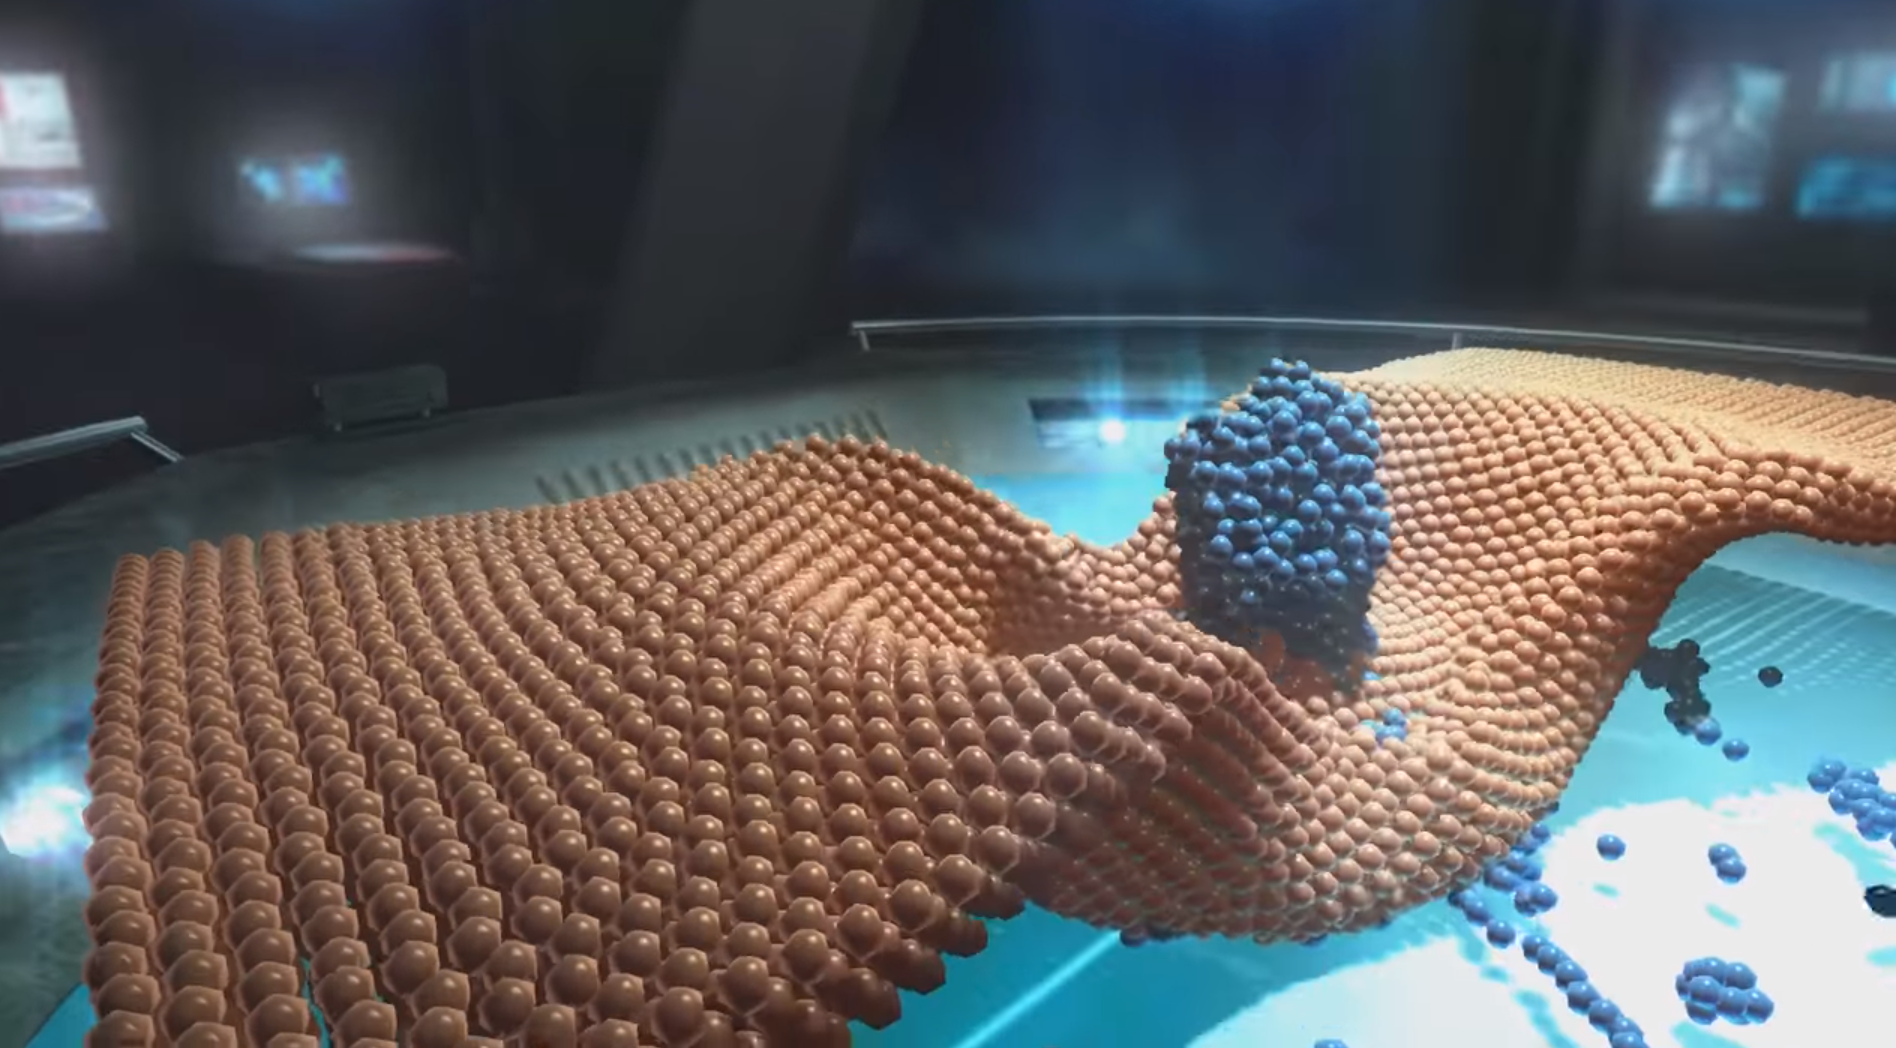
\includegraphics[width=10cm]{archivos/fr-063-magellan}
	\caption{Farbrausch 63: Magellan - Fuente: \href{https://www.youtube.com/watch?v=2Vguvli1Y0k}{YouTube}}
	\label{fig:magellan}
\end{figure}

\subsection{Future Crew}

Future Crew\footnote{\url{https://en.wikipedia.org/wiki/Future_Crew}} fue un grupo de \emph{demosceners} finés, activo principalmente entre 1987 y 1994. Su obra y legado son ampliamente conocidos en el mundo de la \emph{demoscene}. El grupo empezó creando demos para Commodore 64, aunque no tardó en pasar a PC.\\

Su trabajo es especialmente conocido no sólo por su calidad, si no también porque consiguieron resultados que en aquella época parecían imposibles. Su demo, Second Reality [\ref{fig:secondreality}], publicada en julio de 1993, se considera una de las demos más influyentes en la historia de la \emph{demoscene}. Además, el grupo fue coorganizador de la primera edición de la \emph{demoparty} Assembly.\\

\begin{figure}[h]
	\centering
	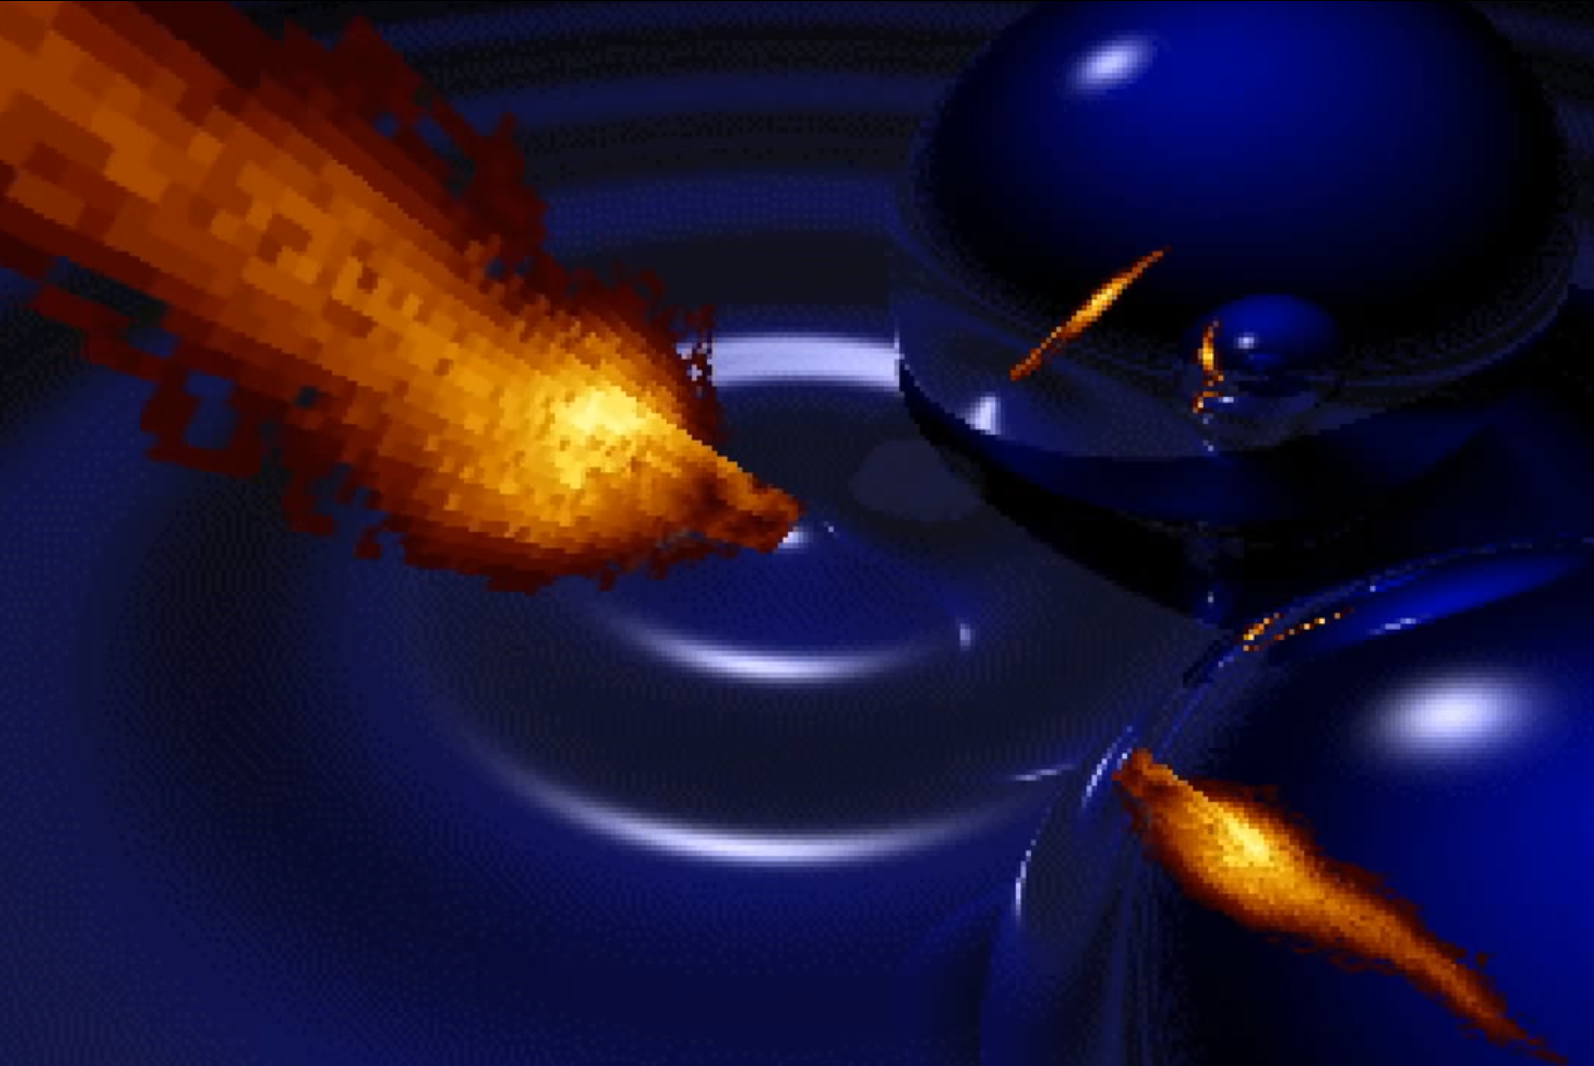
\includegraphics[width=10cm]{archivos/second-reality}
	\caption{Second Reality - Fuente: \href{https://www.youtube.com/watch?v=XezcZVu66QI}{YouTube} - En esta captura se puede ver un efecto de reflexión en dos esferas en tiempo real, mediante \emph{raytracing}}
	\label{fig:secondreality}
\end{figure}

Si bien no se produjo una disolución oficial, el grupo se fue deshaciendo paulatinamente hacia la segunda parte de los 90. La mayoría de sus miembros pasaron a la industria del videojuego o de los gráficos por computador, muchos de ellos fundando sus propios estudios, con resultados exitosos.

\subsection{PoPsY TeAm}

PoPsY TeAm\footnote{\url{http://www.popsyteam.org}} es un grupo de \emph{demosceners} franceses fundado en Lyon, en julio de 1996. Empezaron produciendo demos para Atari y posteriormente para PC.\\

Son los creadores y promotores de VIP (Very Important Party), la \emph{demoparty} más relevante de Francia. Además, PoPsY TeAm se estableció en 2001 como una asociación legalmente registrada en Francia.\\

Su demo más conocida es VIP2 [\ref{fig:vip2}], una demo que presentaron en la \emph{demoparty} holandesa TakeOver en el 2000, resultando ganadora. El objetivo de esta demo era también el de promover su propia \emph{demoparty}, VIP. Esta demo, además, fue la primera de PoPsY TeAm en usar aceleración gráfica por hardware.\\

\begin{figure}[h]
	\centering
	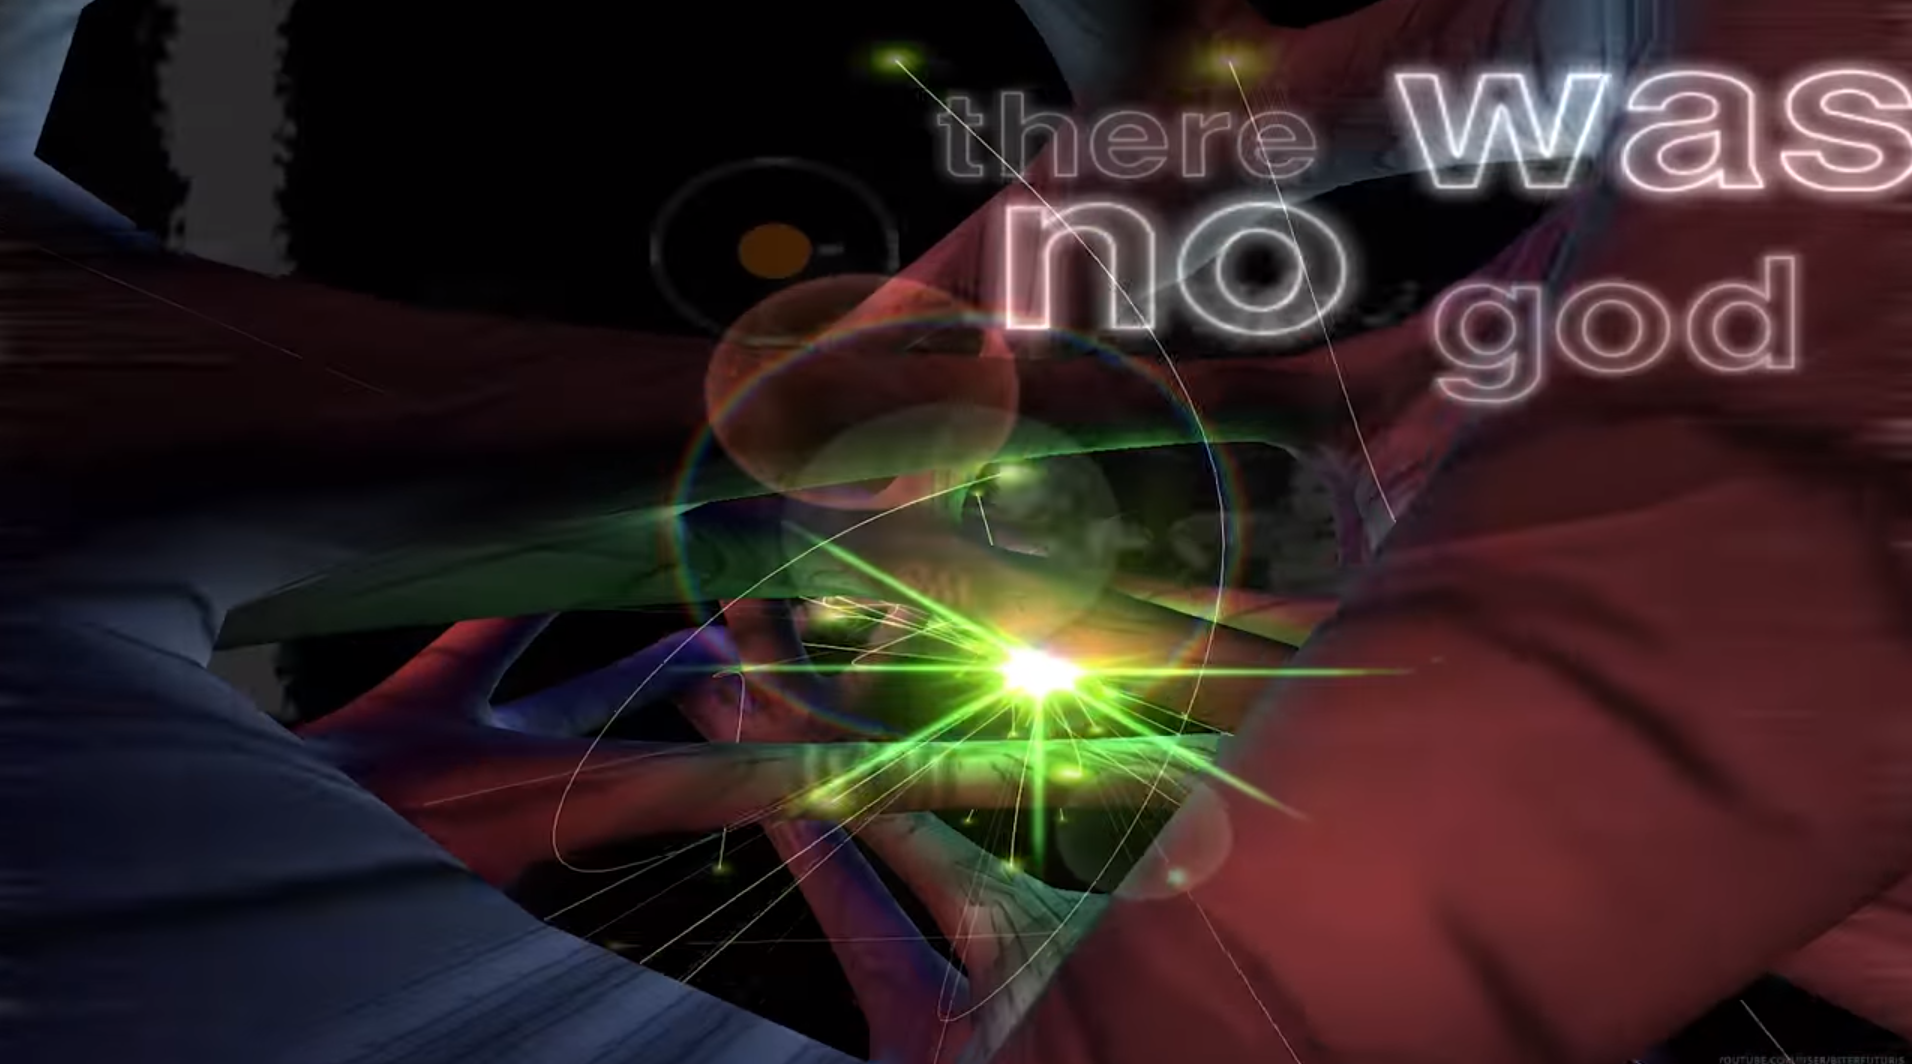
\includegraphics[width=10cm]{archivos/vip2}
	\caption{VIP2 - Fuente: \href{https://www.youtube.com/watch?v=ObtPizPFMbo}{YouTube}}
	\label{fig:vip2}
\end{figure}

El grupo siempre ha intentado promover la \emph{demoscene} y entre otras cosas, han llegado a organizar viajes en bus a diversas partes de Europa para hacer posible al resto de \emph{demosceners} de la región de Lyon atender a \emph{demoparties} europeas. Además, diversos miembros del equipo han participado en la industria del videojuego.

\subsection{Equinox}

Equinox\footnote{\url{https://equinox.planet-d.net}} es un grupo de \emph{demosceners} francés que estuvo principalmente activo entre 1988 y 2007, siendo principalmente conocido por sus demos para Atari ST, aunque sus últimas demos, publicadas pasado el cambio de milenio, fueron lanzadas para PC.

\begin{figure}[h]
	\centering
	\begin{subfigure}[b]{0.45\textwidth}
		\centering
		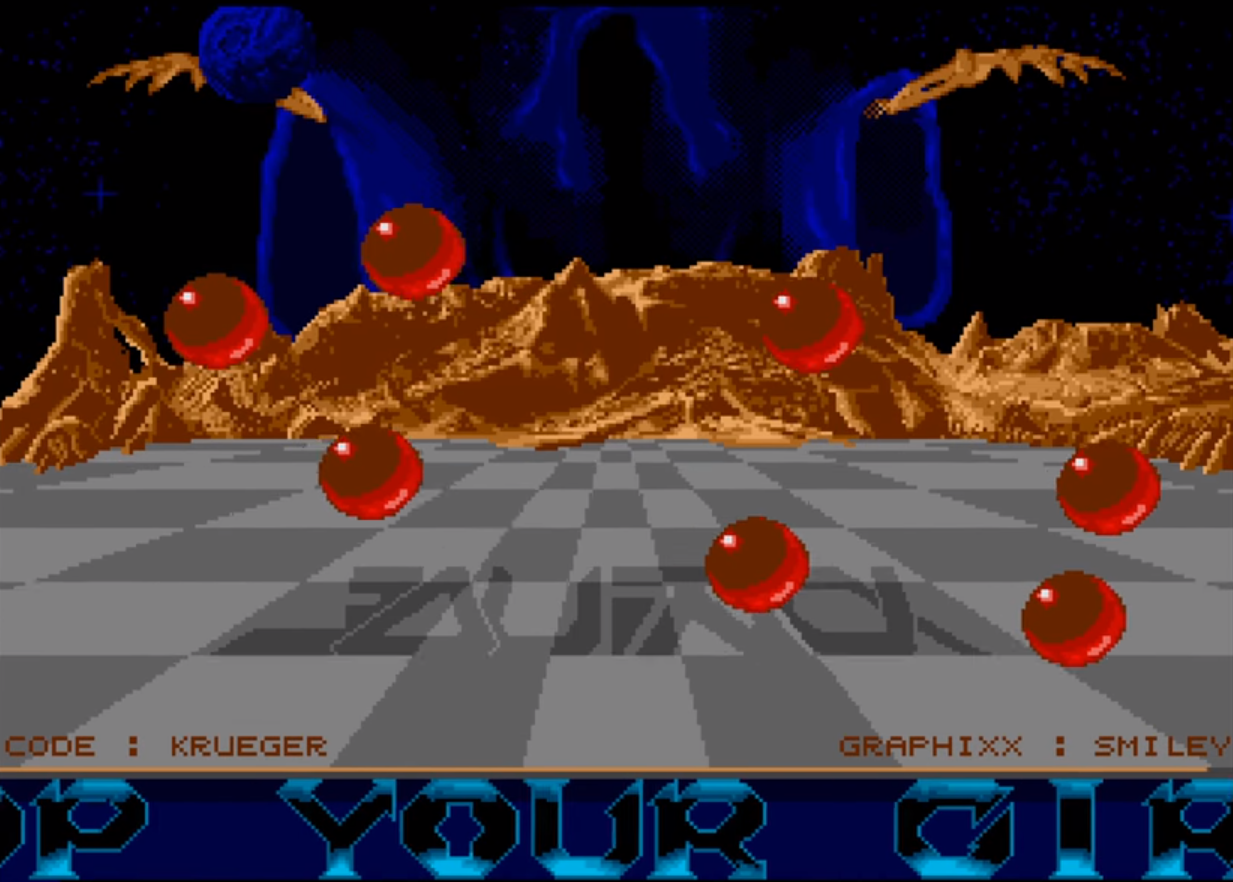
\includegraphics[width=6cm]{archivos/equinox1}
		\caption{Pupul intro (1989) - Fuente : \href{https://www.youtube.com/watch?v=efjEJIj5rhM}{YouTube}}
		\label{fig:equinox1}
	\end{subfigure}
	\begin{subfigure}[b]{0.45\textwidth}
		\centering
		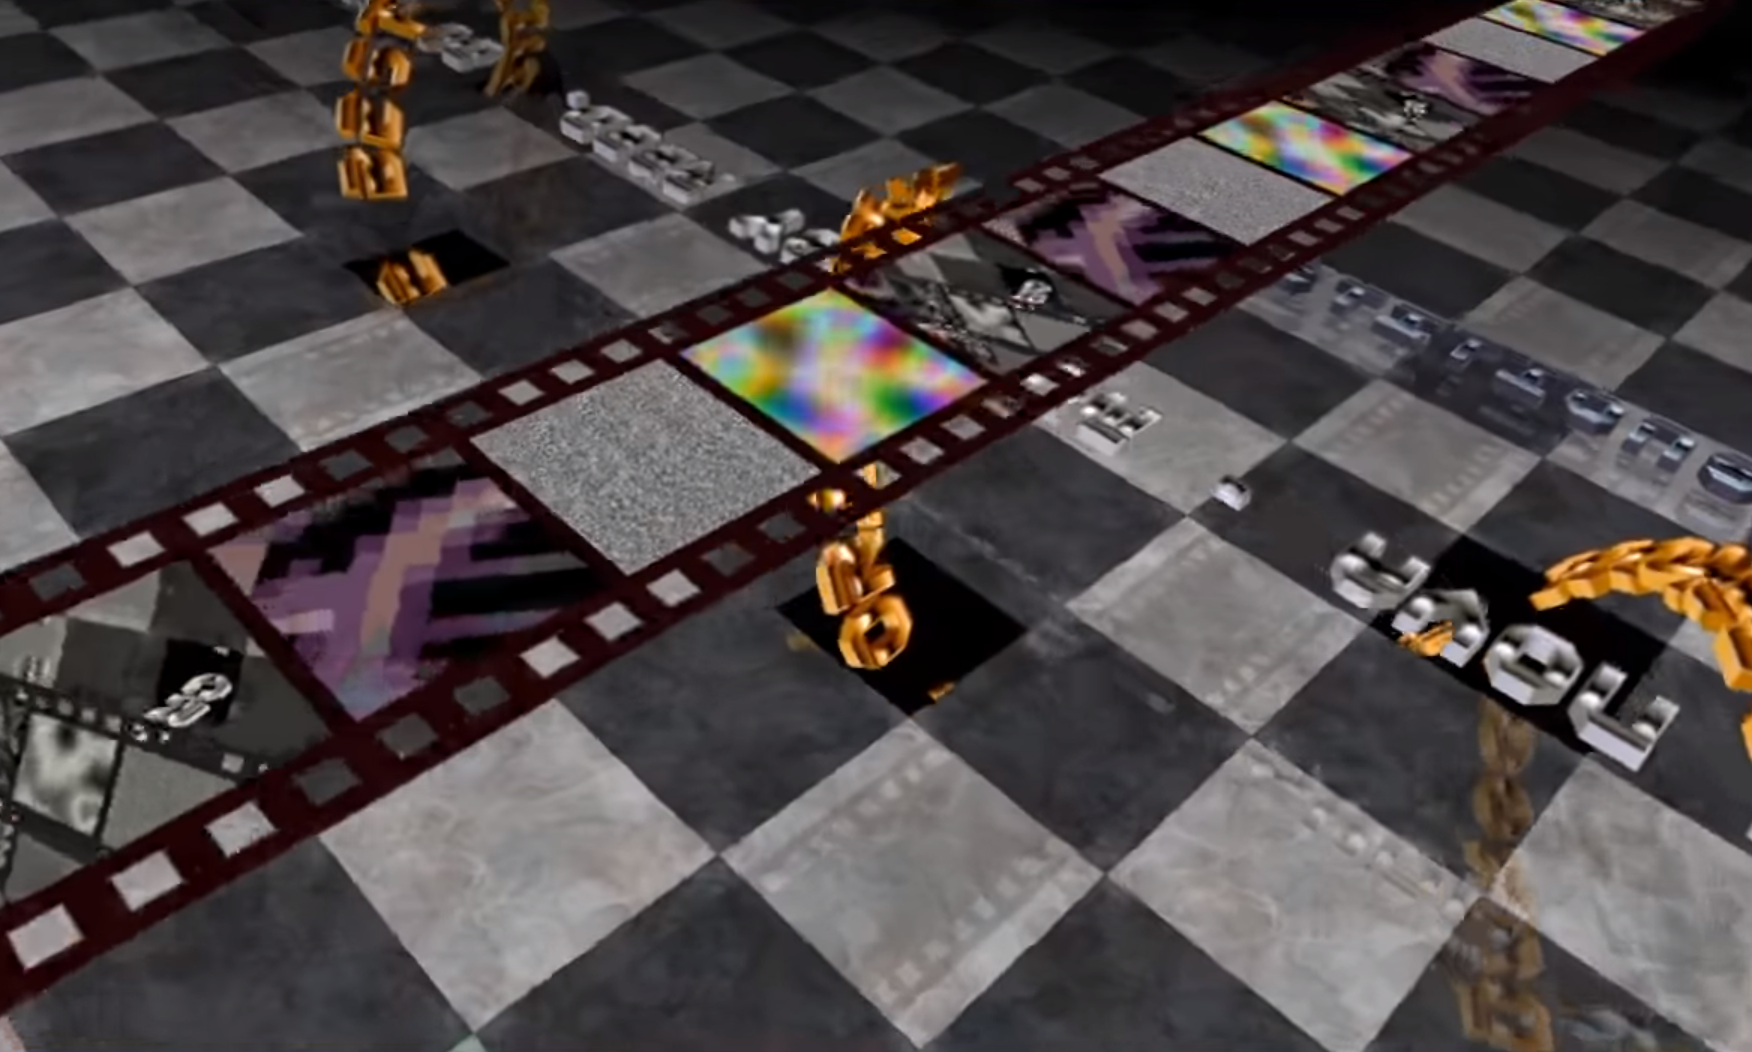
\includegraphics[width=6cm]{archivos/equinox2}
		\caption{Sota 2004 invitation intro (64k intro) - Fuente: \href{https://www.youtube.com/watch?v=cb8i0WYDLxM}{YouTube}}
		\label{fig:equinox2}
	\end{subfigure}
\end{figure}

\subsection{Fairlight}

FairLight\footnote{\url{http://www.fairlight.to}} es un grupo de \emph{demosceners} de origen sueco, formado en 1987. FairLight empezó creando demos para Commodore, aunque ha creado también demos para Amiga, SNES y posteriormente en PC.\\

FairLight fue fundado en 1987 por dos \emph{crackers} suecos, ex-miembros de un grupo llamado "West Coast Crackers". De hecho, FairLight no solo se dedicaba a la \emph{demoscene}, si no también al mundo del \emph{cracking}, rompiendo juegos para su lanzamiento gratuito de forma ilegal. De hecho, llegaron a hacerse especialmente conocidos por la velocidad a la que eran capaces de lanzar juegos \emph{crackeados}\footnote{\url{https://computersweden.idg.se/2.2683/1.444716/we-might-be-old-but-were-still-the-elite}}. Tal fue su impacto que en Abril de 2004, varios miembros del grupo fueron tomados por el FBI en una operación antipiratería denominada \emph{Operation FastLink}. Más de 120 personas fueron arrestadas en esta operación, en la que se consideraba a los \emph{crackers} como una organización criminal.\\

\begin{figure}[h]
	\centering
	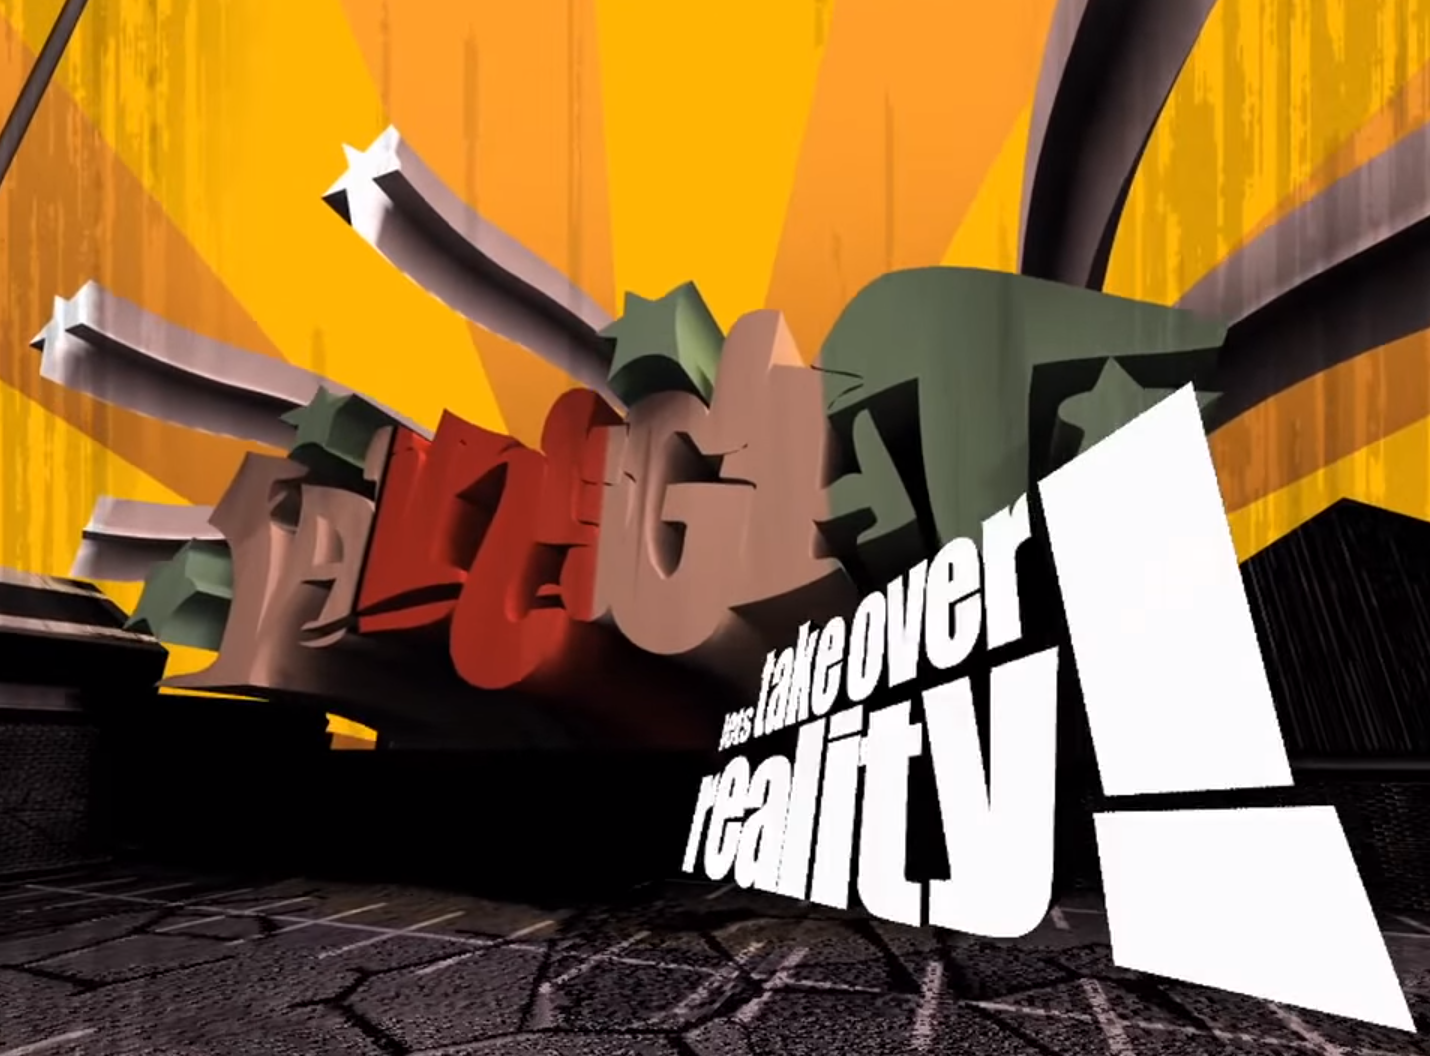
\includegraphics[width=10cm]{archivos/fairlight}
	\caption{Dead Ringer (por FairLight) - Fuente: \href{https://www.youtube.com/watch?v=Mc_TR4mcJKE}{YouTube} - Demo 64k ganadora de Assembly 2006}
	\label{fig:fairlight}
\end{figure}

Este es, quizás, un grupo en el que se reflejan y mezclan los orígenes de la \emph{demoscene}, provenientes del mundo del \emph{cracking}. A pesar de todo, el grupo volvió a estar en activo a partir de octubre de 2006.

\subsection{RGBA}

RGBA\footnote{\url{http://www.rgba.org}} es un grupo español de \emph{demosceners} que estuvo activo entre 2001 y 2009. Todas sus producciones fueron lanzadas para PC, principalmente en Windows.\\

Son especialmente conocidos por su demo Elevated[\ref{fig:elevated}]. Esta demo, realizada en colaboración con TBC\footnote{\url{https://demozoo.org/groups/641/}}, es especialmente conocida y celebrada por la comunidad \emph{demoscener}, situándose como la segunda más popular en el portal \url{http://www.pouet.net}.\\

Los binarios de todas sus producciones se pueden encontrar en \href{https://github.com/reality3d/rgba-prods}{GitHub}.\\

\begin{figure}[h]
	\centering
	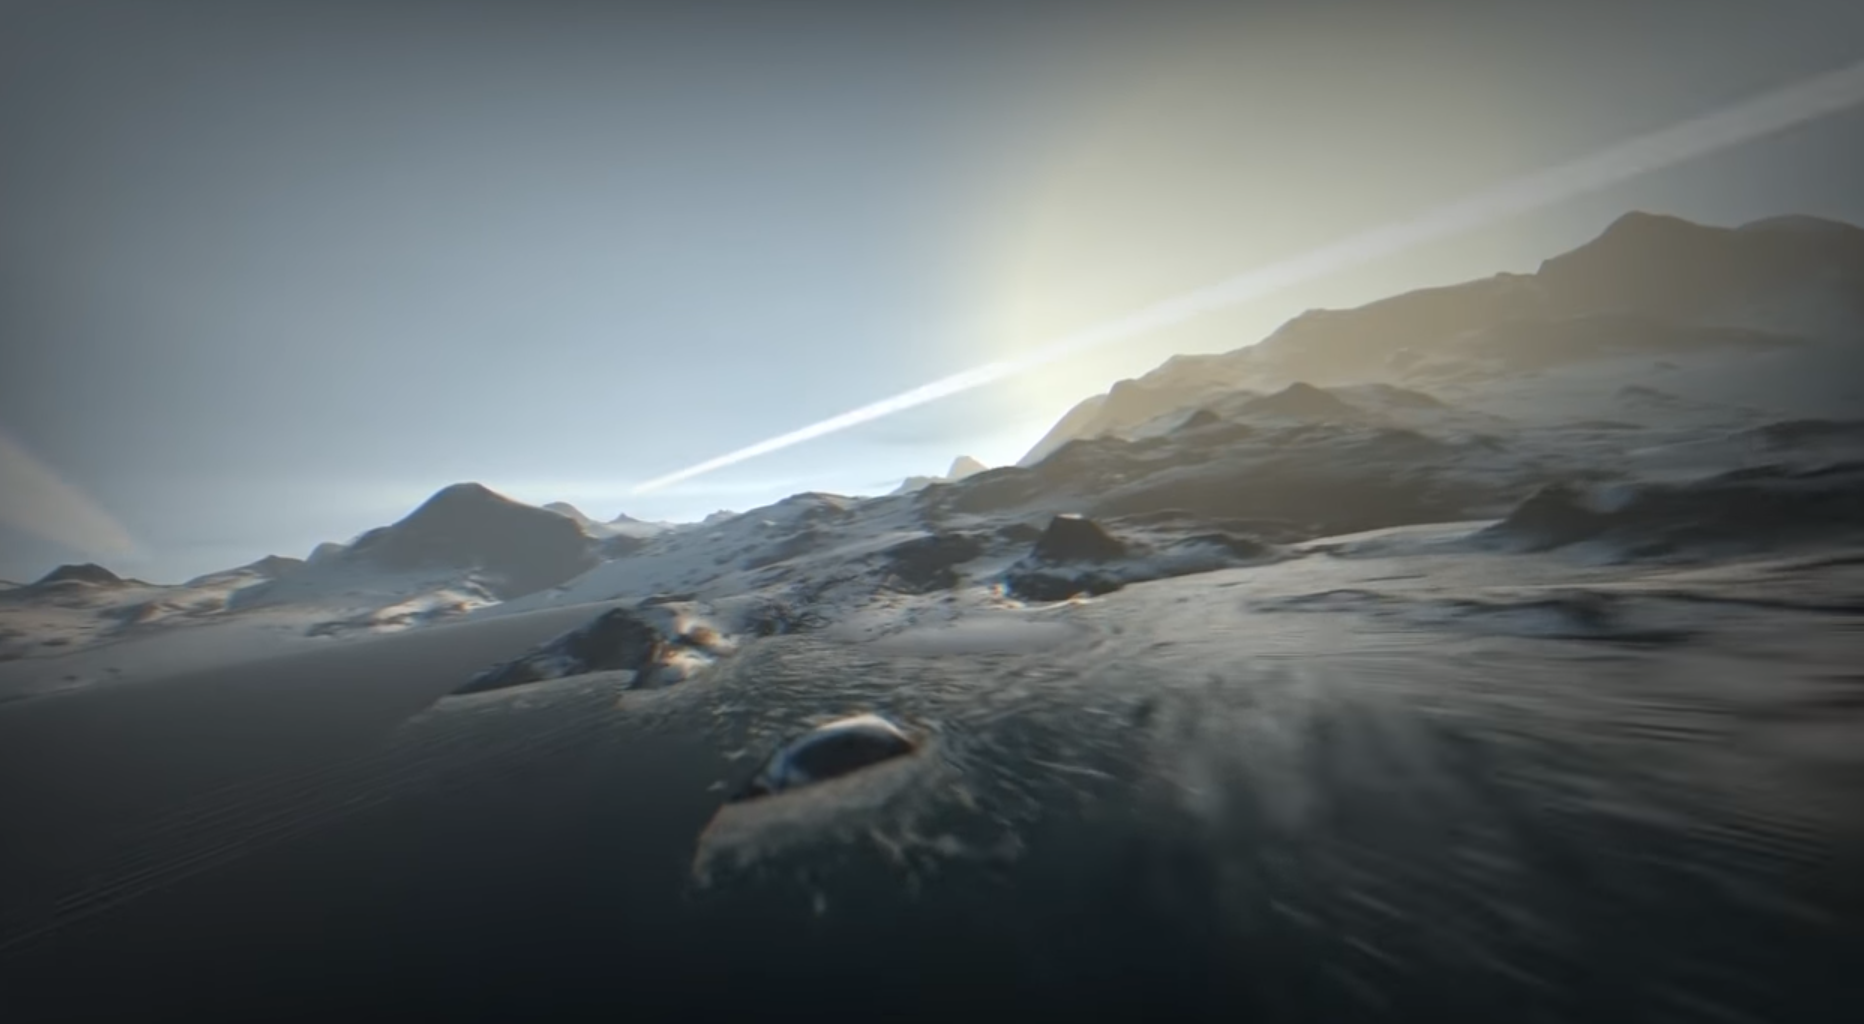
\includegraphics[width=10cm]{archivos/elevated}
	\caption{Elevated - Fuente: \href{https://www.youtube.com/watch?v=jB0vBmiTr6o}{YouTube} - Intro 4K ganadora en Breakpoint 2009}
	\label{fig:elevated}
\end{figure}

\subsection{Batman Group}

Batman Group\footnote{\url{https://demozoo.org/groups/18871/}} es un modesto grupo de \emph{demosceners} de origen español, activo desde 1993. Han producido juegos y demos para Amstrad CPC, ZX Spectrum, Amiga, Android e iOS.\\

Su demo más conocida es Batman Forever[\ref{fig:batmanforever}], para Amstrad CPC, lanzada en 2011 para la \emph{demoparty} eslovaca Forever, quedando en primera posición.\\

\begin{figure}[h]
	\centering
	
\includegraphics[width=10cm]{archivos/batmanforever}
	\caption{Batman Forever - Fuente: \href{https://www.youtube.com/watch?v=dqjZNnjNu3Y}{YouTube}}
	\label{fig:batmanforever}
\end{figure}

El grupo se vio envuelto en una polémica a finales de 2018, debido a que el grupo de desarrolladores retro \emph{4MHz} había usado para sus producciones código cedido por Batman Group sin su correcta atribución. La polémica se resolvió con la disolución de todo tipo de relación entre Batman Group y 4MHz\footnote{\url{http://www.amstrad.es/forum/viewtopic.php?t=5247}}.

\section{Portales de demoscening}

A continuación se listan y describen algunos de los portales más populares dedicados a la \emph{demoscene}. Estos portales surgen de la pasión por la \emph{demoscene}, pero son a su vez una interesante y valiosa fuente de conocimiento, así como un reflejo de la historia y el avance de la computación desde finales de los años 80 hasta la actualidad.

\begin{itemize}
	\item \textbf{\href{https://www.scene.org}{Scene.org}}: el portal y archivo de la \emph{demoscene} por excelencia. El archivo de Scene.org contiene una cantidad inmensa y de lo más completa de demos. En resumen, si estás buscando una demo específica, lo más probable es que esté alojada aquí.
	\item \textbf{\href{http://www.pouet.net}{Pouet}}: el mayor foro dedicado de forma exclusiva a la \emph{demoscene}. Prácticamente cualquier demo que se produce es subida a esta página, donde puede ser votada y comentada por la comunidad. El sitio aloja más de 75000 producciones, y contiene ránkings de las mejores demos de todos los tiempos, votadas por los usuarios.
	\item \textbf{\href{https://demozoo.org}{Demozoo}}: portal dedicado a la \emph{demoscene} que aloja una gran cantidad de información sobre \emph{demogroups} y sus producciones.
	\item \textbf{\href{http://www.slengpung.com}{Slengpung}}: este es un curioso portal dedicado a recopilar fotografías tomadas en \emph{demoparties}. Si se ha sido fotografiado en un evento relacionado con la \emph{demoscene}, lo más probable es que se pueda encontrar la imagen en este sitio. Contiene tanto imágenes con más de 25 años de antigüedad como otras tomadas en las \emph{demoparties} más recientes. Este sitio permite además familiarizarse con la cultura de la \emph{demoscene} desde el punto de vista más social y observar su evolución a lo largo del tiempo.
	\item \textbf{\href{https://www.hornet.org}{Hornet}}: se trata de un archivo de la \emph{demoscene} para PC entre 1992 y 1998. Contiene más de 16000 documentos, en un total de más de 7GB. Al tratarse de un archivo, es difícil navegar o encontrar información en él, pero vale la pena dedicar un rato a perderse entre sus ficheros. Este sitio contiene una gran cantidad de conocimiento y pasión, incluyendo acceso a un magazine semanal que llegó a publicar 150 números. Este semanario contenía entrevistas, resúmenes de eventos, explicaciones matemáticas sobre demos y un sinfín más de información.
	\item \textbf{\href{http://www.oldskool.org}{OldSkool}}: este portal está dedicado en general a la nostalgia por los PCs y la programación de la "vieja escuela". Es una fuente de recursos que da acceso a información sobre el lado más clásico de la \emph{demoscene}.
	\item \textbf{\href{http://www.demoscene.info}{Demoscene.info}}: pequeño portal que contiene información acerca de otros sitios, eventos, demos y \emph{demogroups}. Es un sitio muy pequeño y sencillo, lo que lo convierte en un buen lugar de referencia para empezar a introducirse en el mundo de la \emph{demoscene}. 
	\item \textbf{\href{http://wanted.scene.org}{Wanted}}: este sitio está pensado para que aquellos \emph{demosceners} que estén buscando a otras personas para su grupo puedan anunciarse, así como para que gente sin grupo pueda anunciar sus intereses y habilidades para ser reclutados. Establece un entorno perfecto para formar o completar grupos de \emph{demosceners}. En otras palabras, podría definirse como el LinkedIn de la \emph{demoscene}.
	\item \textbf{\href{https://www.demoparty.net}{Demoparty.net}}: pequeño y sencillo portal que lista las próximas \emph{demoparties} y eventos en Europa.
	\item \textbf{\href{http://curio.scene.org}{Curio}}: archivo dedicado a la \emph{demoscene} moderna. Si se busca ver lo último en efectos y gráficos en tiempo real, este es el lugar adecuado.
	\item \textbf{\href{https://id.scene.org}{SceneID}}: este es un curioso portal. Ofrece un servicio de autenticación común para los portales de \emph{demoscene}. Gracias a este servicio, es posible acceder a los principales portales de la \emph{demoscene} bajo los mismos credenciales.
\end{itemize}

\section{Demos destacables}
juntar y hablar de las principales demos en la demoscene, hacer referencia al top de pouet, incluir elevated y otras mas e intentar explicarlas

\section{Efectos gráficos más comunes}

A continuación se listan algunos de los efectos clásicos más comunes. Estos son efectos gráficos que llevan presentes desde el inicio de la \emph{demoscene} y que se pueden ver en una gran cantidad de producciones \footnote{\url{http://www.oldskool.org/demos/explained/demo_graphics.html}} \footnote{\url{http://demo-effects.sourceforge.net}} \footnote{\url{https://en.wikipedia.org/wiki/Demo_effect}}.

\begin{itemize}
	\item \textbf{Fuego}: efecto clásico por excelencia [\ref{fig:fire_inconexia}], podría considerarse casi el "Hola Mundo" de la \emph{demoscene}, debido a su sencillo pero consistente resultado. El efecto de fuego en tiempo real es muy sencillo a nivel de implementación, aunque computacionalmente costoso.
	\item \textbf{Plasma}: este efecto es otro de los grandes clásicos [\ref{fig:plasma}]. Es nuevamente un efecto muy sencillo de implementar, pero con alto coste computacional, por lo que normalmente son necesarias optimizaciones o aproximaciones. Puede implementarse mediante la combinación de funciones de seno o mediante funciones de ruido.
	\item \textbf{Partículas}: un tipo de efecto muy socorrido es el de partículas. Debido a las limitaciones de los ordenadores, tener que actualizar miles de píxeles en pantalla, a veces con operaciones matemáticas complejas de por medio, era muy a menudo inviable. Sin embargo, aplicar efectos con trayectorias o transformaciones complejas a sets reducidos de objetos (partículas) en pantalla era perfectamente viable. En esta demo de Equinox [\ref{fig:equinox1}] cada una de las esferas se podría considerar de hecho una partícula con una trayectoria compleja. \\
	Otro uso muy común era el de crear "nubes de puntos". Eran efectos como túneles o formas de apariencia tridimensional compleja (como paraboloides) formados por puntos. La aplicación de estas fórmulas píxel a píxel era computacionalmente inviable, sin embargo, al aplicarlas únicamente sobre un set reducido de píxeles, podían lograrse resultados en tiempo real de lo más sorprendentes\footnote{\url{https://www.youtube.com/watch?v=L_xycbyI1vU}}.
	\item \textbf{Deformaciones de imagen}: las deformaciones de imagen son y han sido efectos muy usados en la demoscene. Muchas de estos tipos de transformación tienen incluso nombre propios. Uno de los efectos más conocidos es el rotozoom (textura que rota y escala simultáneamente) y se logra mediante la aplicación de transformaciones de escalado (multiplicaciones) y transformaciones de rotación (senos y cosenos). Otros efectos de deformación muy populares son las deformaciones de lente o las torsiones [\ref{fig:deformaciones}].
	\item \textbf{Vectores y geometría}: hoy en día, puede que los entornos virtuales en 3D se den como algo garantizado, pero detrás de ello lo único que hay son transformaciones matemáticas mediante el uso de matrices y vectores. Cuando no había tarjetas gráficas ni librerías para gráficos 3D, crear figuras geométricas con sensación de tridimensionalidad era todo un reto, no hablemos ya de escenas complejas [\ref{fig:vectorworld}].
	\item \textbf{Raytracing}: el \emph{raytracing} es una técnica de iluminación usada especialmente para el cálculo de reflexiones. Esta técnica consiste básicamente en hallar la trayectoria de la luz lanzando haces de rayos. Hoy en día existen muchos algoritmos de \emph{raytracing}, y aún así, sigue siendo una operación computacionalmente costosa. Sin embargo, se puede encontrar demos de hace más de 20 años que ya conseguían aplicar esta técnica en tiempo real [\ref{fig:secondreality}].
	\item \textbf{Otros}: existen una infinidad de efectos y variaciones más. Entre otras destacan los efectos de planos infinitos (mediante el uso de transformaciones afines, es conocido como el Modo 7 \footnote{\url{https://en.wikipedia.org/wiki/Mode_7}} de Nintendo, usado en juegos como el Mario Kart de la Super Nintendo). El efecto de planos infinitos emula un entorno 3D mediante el uso de una textura 2D.
\end{itemize}

\begin{figure}[h]
	\centering
	\begin{subfigure}[b]{0.45\textwidth}
		\centering
		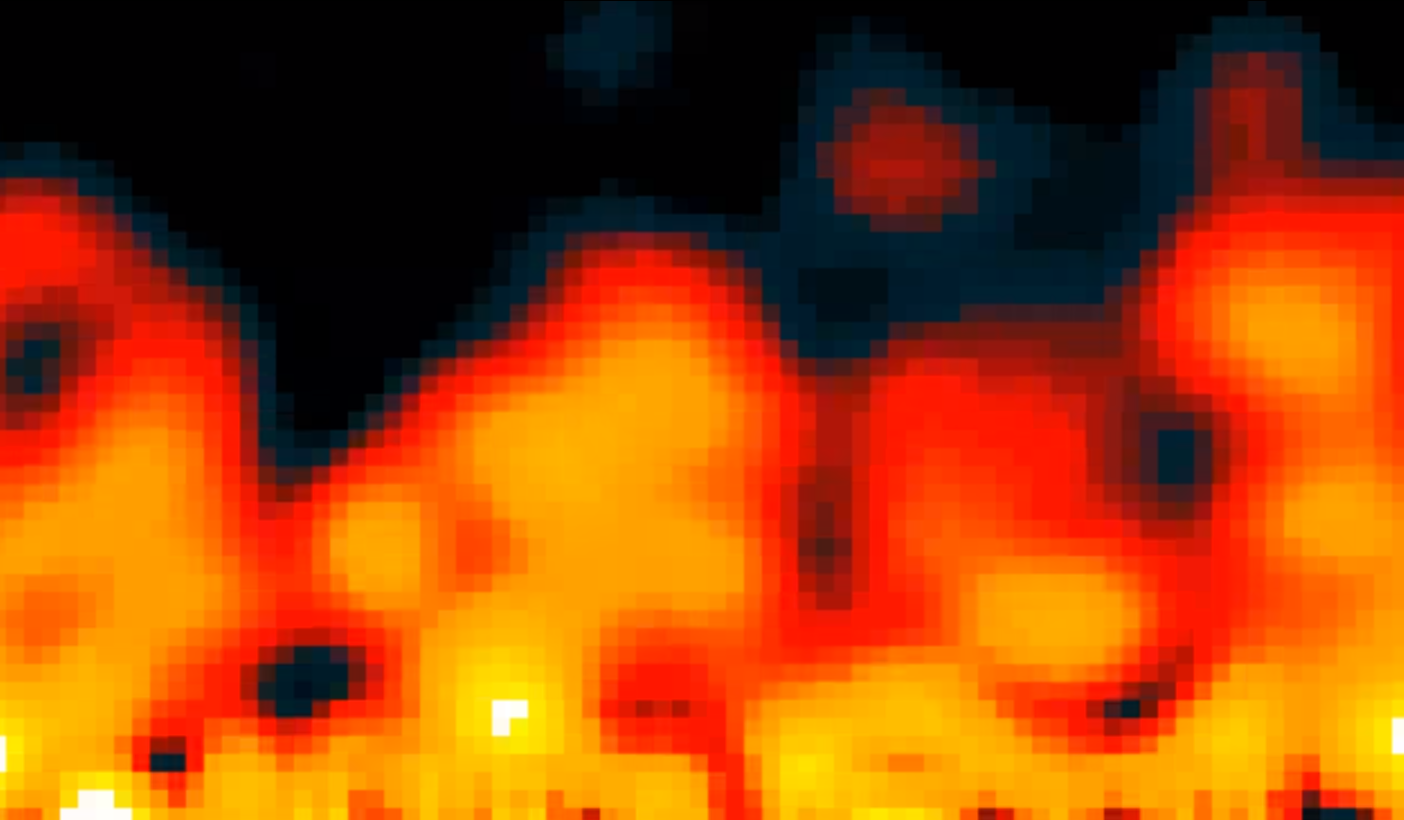
\includegraphics[width=6cm]{archivos/fire_inconexia}
		\caption{Efecto de fuego - Inconexia (por Iguana) - Fuente : \href{https://www.youtube.com/watch?v=ztxbEbUa4YY}{YouTube}}
		\label{fig:fire_inconexia}
	\end{subfigure}
	\begin{subfigure}[b]{0.45\textwidth}
		\centering
		
\includegraphics[width=6cm]{archivos/plasma}
		\caption{Efecto de plasma - Fuente : \href{https://en.wikipedia.org/wiki/Plasma_effect\#/media/File:Plasma_effect.jpg}{Wikipedia}}
		\label{fig:plasma}
	\end{subfigure}
	\begin{subfigure}[b]{0.45\textwidth}
		\centering
		
\includegraphics[width=6cm]{archivos/deformaciones}
		\caption{Deformación de imagen - Batman Forever (por Batman Group) - Fuente: \href{https://www.youtube.com/watch?v=YJosZfm560Q}{YouTube}}
		\label{fig:deformaciones}
	\end{subfigure}
	\begin{subfigure}[b]{0.45\textwidth}
		\centering
		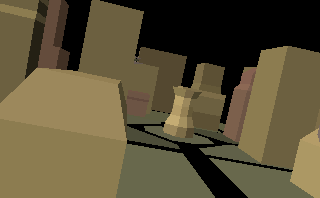
\includegraphics[width=6cm]{archivos/vectorworld}
		\caption{Mundo vectorial - Airframe (por Prime) - Fuente: \href{http://www.oldskool.org/demos/explained/htmlpictures/vectorw.gif}{OldSkool}}
		\label{fig:vectorworld}
	\end{subfigure}
\end{figure}



%http://www.farbrausch.de/index.py https://en.wikipedia.org/wiki/Farbrausch
%https://en.wikipedia.org/wiki/Future_Crew https://demozoo.org/groups/357/
%http://www.popsyteam.org https://en.wikipedia.org/wiki/Very_Important_Party
%https://en.wikipedia.org/wiki/Equinox_(Atari_demogroup) https://equinox.planet-d.net/atari.html
%https://demozoo.org/groups/18871/
%https://en.wikipedia.org/wiki/Fairlight_(group)

\section{Influencia de la demoscene en la industria}

La \emph{demoscene} siempre se ha mantenido de forma discreta. Algunas de las razones de que esto sea así se han listado anteriormente, como el hecho de que hace una gran cantidad de conocimiento y pasión para poder participar de forma activa en ella. Sin embargo, esto no ha impedido dejar su huella en la industria informática, especialmente en la del videojuego.\\

La lista de personalidades que vienen del mundo de la \emph{demoscene} o se han visto influidos por ella es extensa\footnote{\url{https://chipflip.wordpress.com/2015/06/12/famous-people-who-came-from-the-demoscene/}}. A continuación se listan algunas de las más destacables:

\begin{itemize}
	\item \textbf{DICE}\footnote{\url{http://www.dice.se}}: La compañía \emph{Digital Illusions}, conocida por juegos como varios de los títulos de la saga \emph{Battefield} o \emph{Mirror's Edge Catalyst}, cuenta con una gran plantilla proveniente de la \emph{demoscene}, entre los que podemos contar miembros de FairLight.
	\item \textbf{Remedy}\footnote{\url{https://www.remedygames.com/}}: Esta compañía es especialmente conocida por la saga Max Payne. Fue cofundada por dos miembros de Future Crew. Además, esta compañía mantenía una estrecha relación con Futuremark, creadores de 3DMark, un software de pruebas de rendimiento (\emph{benchmarks}). Esta última compañía también poseía una gran cantidad de miembros provenientes de la \emph{demoscene}, contando con varios de Future Crew.
	\item \textbf{Starbreeze, Ascaron, 49Games, Techland, Lionhead Studios, Guerrilla Games}: Todas estas compañías también cuentan o han contado con miembros de la \emph{demoscene}.
	\item Will Wright, creador del vieojuego Spore, afirma que la \emph{demoscene} fue una gran influencia para al juego, debido a que este está fundamentalmente basado en la generación procedimental de contenido\footnote{\url{http://www.gamespy.com/articles/595/595975p1.html}}.
	\item John Carmack, \emph{lead programmer} de videojuegos como Wolfestein 3D, Doom y Quake, afirmó en la QuakeCon de 2011 que tiene en alta consideración a aquellos programadores que desarrollan demos de 64K, pues tienen que hacer frente a grandes limitaciones y se obtiene mucho conocimiento en el proceso\footnote{\url{https://www.youtube.com/watch?v=4zgYG-_ha28\#t=4827s}}.
	\item Jaakko Iisalo, principal diseñador de Angry Birds, fue un \emph{demoscener} activo y reconocido durante los 90.
\end{itemize}

Además, hay algunas otras subculturas informáticas que están estrechamente relacionadas con la \emph{demoscene} o derivan de la misma, como por ejemplo la música por \emph{tracker} (hay toda una comunidad de músicos que crean producciones a través del uso de \emph{trackers}, software para la producción de música).

%Importantes para la historia:
%http://widerscreen.fi/assets/reunanen-wider-1-2-2014.pdf
%http://www.oldskool.org/demos/explained/demo_history.html
%https://web.archive.org/web/20170726063815/http://tomaes.32x.de/text/faq.php#2.3.

%Elevated y otras demos por el estilo

%https://web.archive.org/web/20170726063815/http://tomaes.32x.de/text/faq.php
%http://www.oldskool.org/demos/explained/demo_history.html

%http://www.oldskool.org/demos/explained/demo_reference.html

%http://www.demoscene.info
%http://www.pouet.net/index.php
%https://en.wikipedia.org/wiki/Assembly_(demoparty)
%https://en.wikipedia.org/wiki/Demoscene

%http://widerscreen.fi/numerot/2014-1-2/crackers-became-us-demosceners/
%http://www.oldskool.org/demos/explained/demo_pages.html
%ftp://ftp.hornet.org/pub/demos/info/demonews/1998/demonews.150

%http://www.farbrausch.de/index.py 
%https://en.wikipedia.org/wiki/Farbrausch
%https://en.wikipedia.org/wiki/Future_Crew 
%https://demozoo.org/groups/357/
%http://www.popsyteam.org 
%https://en.wikipedia.org/wiki/Very_Important_Party
%https://en.wikipedia.org/wiki/Equinox_(Atari_demogroup) 
%https://equinox.planet-d.net/atari.html
%https://demozoo.org/groups/18871/